% Soubory musí být v kódování, které je nastaveno v příkazu \usepackage[...]{inputenc}

\documentclass[%
%  draft,    				  % Testovací překlad
  12pt,       				% Velikost základního písma je 12 bodů
  a4paper,    				% Formát papíru je A4
%  oneside,      			% Jednostranný tisk (výchozí)
%% Z následujicich voleb lze použít maximálně jednu:
%	dvipdfm  						% výstup bude zpracován programem 'dvipdfm' do PDF
%	dvips	  						% výstup bude zpracován programem 'dvips' do PS
%	pdftex							% překlad bude proveden programem 'pdftex' do PDF (výchozí)
	unicode,						% Záložky a informace budou v kódování unicode
%% Z následujících voleb lze použít jen jednu:
%english,            % originální jazyk je angličtina
czech              % originální jazyk je čeština (výchozí)
%slovak,             % originální jazyk je slovenčina
]{report}				    	% Dokument třídy 'zpráva'

\usepackage[utf8]		%	Kódování zdrojových souborů je v UTF-8
	{inputenc}					% Balíček pro nastavení kódování zdrojových souborů

\usepackage{graphicx} % Balíček 'graphicx' pro vkládání obrázků
											% Nutné pro vložení log školy a fakulty

\usepackage[
	nohyperlinks				% Nebudou tvořeny hypertextové odkazy do seznamu zkratek
]{acronym}						% Balíček 'acronym' pro sazby zkratek a symbolů
											% Nutné pro použití prostředí 'seznamzkratek' balíčku 'thesis'

\usepackage[
	breaklinks=true,		% Hypertextové odkazy mohou obsahovat zalomení řádku
	hypertexnames=false % Názvy hypertextových odkazů budou tvořeny
											% nezávisle na názvech TeXu
]{hyperref}						% Balíček 'hyperref' pro sazbu hypertextových odkazů
											% Nutné pro použití příkazu 'nastavenipdf' balíčku 'thesis'

\usepackage{pdfpages} % Balíček umožňující vkládat stránky z PDF souborů
                      % Nutné při vkládání titulních listů a zadání přímo
                      % ve formátu PDF z informačního systému

\usepackage{enumitem} % Balíček pro nastavení mezerování v odrážkách
  \setlist{topsep=0pt,partopsep=0pt,noitemsep}

\usepackage{cmap} 		% Balíček cmap zajišťuje, že PDF vytvořené `pdflatexem' je
											% plně "prohledávatelné" a "kopírovatelné"

\usepackage{upgreek}	% Balíček pro sazbu stojatých řeckých písmem
											% např. stojaté pí: \uppi
											% např. stojaté mí: \upmu (použitelné třeba v mikrometrech)
											% pozor, grafická nekompatibilita s fonty typu Computer Modern!

\usepackage{dirtree}		% sazba adresářové struktury

\usepackage[formats]{listings}	% Balíček pro sazbu zdrojových textů
\lstset{
%	Definice jazyka použitého ve výpisech
%    language=[LaTeX]{TeX},	% LaTeX
%	language={Matlab},		% Matlab
	language={C},           % jazyk C
    basicstyle=\ttfamily,	% definice základního stylu písma
    tabsize=2,			% definice velikosti tabulátoru
    inputencoding=utf8,         % pro soubory uložené v kódování UTF-8
    %inputencoding=cp1250,      % pro soubory uložené ve standardním kódování Windows CP1250
		columns=fixed,  %flexible,
		fontadjust=true %licovani sloupcu
    extendedchars=true,
    literate=%  definice symbolů s diakritikou
    {á}{{\'a}}1
    {č}{{\v{c}}}1
    {ď}{{\v{d}}}1
    {é}{{\'e}}1
    {ě}{{\v{e}}}1
    {í}{{\'i}}1
    {ň}{{\v{n}}}1
    {ó}{{\'o}}1
    {ř}{{\v{r}}}1
    {š}{{\v{s}}}1
    {ť}{{\v{t}}}1
    {ú}{{\'u}}1
    {ů}{{\r{u}}}1
    {ý}{{\'y}}1
    {ž}{{\v{z}}}1
    {Á}{{\'A}}1
    {Č}{{\v{C}}}1
    {Ď}{{\v{D}}}1
    {É}{{\'E}}1
    {Ě}{{\v{E}}}1
    {Í}{{\'I}}1
    {Ň}{{\v{N}}}1
    {Ó}{{\'O}}1
    {Ř}{{\v{R}}}1
    {Š}{{\v{S}}}1
    {Ť}{{\v{T}}}1
    {Ú}{{\'U}}1
    {Ů}{{\r{U}}}1
    {Ý}{{\'Y}}1
    {Ž}{{\v{Z}}}1
}

%% Nastavení českého jazyka při sazbě v češtině.
% Pro sazbu češtiny je možné použít mezinárodní balíček 'babel', jenž
% použití doporučujeme pro nové instalace (MikTeX2.8,TeXLive2009), nebo
% národní balíček 'czech', který doporučujeme ve starších instalacích.
% Balíček 'babel' bude správně fungovat pouze ve spojení s programy
% 'latex', 'pdflatex', zatímco balíček 'czech' bude fungovat ve spojení
% s programy 'cslatex', 'pdfcslatex'.
% Varianta A:
\usepackage    				
  {babel}             % Balíček pro sazbu různojazyčných dokumentů; kompilovat (pdf)latexem!
  										% převezme si z parametrů třídy správný jazyk
\usepackage{lmodern}	% vektorové fonty Latin Modern, nástupce půvoních Knuthových Computern Modern fontů
\usepackage{textcomp} % Dodatečné symboly
\usepackage[T1]{fontenc}  % Kódování fontu - mj. kvůli správným vzorům pro dělení slov
% Varianta B:
%\usepackage{czech}   % Alternativní balíček pro sazbu v českém jazyce, kompilovat (pdf)cslatexem!

\usepackage[%
%% Z následujících voleb lze použít pouze jednu
% left,               % Rovnice a popisky plovoucich objektů budou %zarovnány vlevo
  center,             % Rovnice a popisky plovoucich objektů budou zarovnány na střed (vychozi)
%% Z následujících voleb lze použít pouze jednu
semestral						%	sazba zprávy semestrálního projektu
%bachelor						%	sazba bakalářské práce
%diploma						 % sazba diplomové práce
%treatise            % sazba pojednání o dizertační práci
%phd                 % sazba dizertační práce
]{thesis}             % Balíček pro sazbu studentských prací
                      % Musí být vložen až jako poslední, aby
                      % ostatní balíčky nepřepisovaly jeho příkazy

%%%%%%%%%%%%%%%%%%%%%%%%%%%%%%%%%%%%%%%%%%%%%%%%%%%%%%%%%%%%%%%%%
%%%%%%      Definice informací o dokumentu             %%%%%%%%%%
%%%%%%%%%%%%%%%%%%%%%%%%%%%%%%%%%%%%%%%%%%%%%%%%%%%%%%%%%%%%%%%%%

%% Název práce:
%  První parametr je název v originálním jazyce,
%  druhý je překlad v angličtině nebo češtině (pokud je originální jazyk angličtina)
\nazev{Nástroje pro předzpracování rentgenových snímků}{Radiography preprocessing tools}

%% Jméno a příjmení autora ve tvaru
%  [tituly před jménem]{Křestní}{Příjmení}[tituly za jménem]
\autor[Bc.]{Petr}{Chmelař}

%% Jméno a příjmení vedoucího/školitele včetně titulů
%  [tituly před jménem]{Křestní}{Příjmení}[tituly za jménem]
% Pokud osoba nemá titul za jménem, smažte celý řetězec '[...]'
\vedouci[Ing.]{Petr}{Petyovský}[Ph.D.]

%% Jméno a příjmení oponenta včetně titulů
%  [tituly před jménem]{Křestní}{Příjmení}[tituly za jménem]
% Pokud nemá titul za jménem, smažte celý řetězec '[...]'
% Uplatní se pouze v prezentaci k obhajobě;
% v případě, že nechcete, aby se na titulním snímku prezentace zobrazoval oponent, pouze jej zakomentujte;
% u obhajoby semestrální práce se oponent nezobrazuje
\oponent[doc.\ Mgr.]{Křestní}{Příjmení}[Ph.D.]

%% Označení oboru studia
% První parametr je obor v originálním jazyce,
% druhý parametr je překlad v angličtině nebo češtině
\oborstudia{Kybernetika, automatizace a měření}{Cybernetics, Control and Measurements}

%% Označení fakulty
% První parametr je název fakulty v originálním jazyce,
% druhý parametr je překlad v angličtině nebo v češtině
%\fakulta{Fakulta architektury}{Faculty of Architecture}
\fakulta{Fakulta elektrotechniky a komunikačních technologií}{Faculty of Electrical Engineering and Communication}
%\fakulta{Fakulta chemická}{Faculty of Chemistry}
%\fakulta{Fakulta informačních technologií}{Faculty of Information Technology}
%\fakulta{Fakulta podnikatelská}{Faculty of Business and Management}
%\fakulta{Fakulta stavební}{Faculty of Civil Engineering}
%\fakulta{Fakulta strojního inženýrství}{Faculty of Mechanical Engineering}
%\fakulta{Fakulta výtvarných umění}{Faculty of Fine Arts}

%% Označení ústavu
% První parametr je název ústavu v originálním jazyce,
% druhý parametr je překlad v angličtině nebo češtině
\ustav{Ústav automatizace a měřicí techniky}{Department of Control and Instrumentation}
%\ustav{Ústav biomedicínského inženýrství}{Department of Biomedical Engineering}
%\ustav{Ústav elektroenergetiky}{Department of Electrical Power Engineering}
%\ustav{Ústav elektrotechnologie}{Department of Electrical and Electronic Technology}
%\ustav{Ústav fyziky}{Department of Physics}
%\ustav{Ústav jazyků}{Department of Foreign Languages}
%\ustav{Ústav matematiky}{Department of Mathematics}
%\ustav{Ústav mikroelektroniky}{Department of Microelectronics}
%\ustav{Ústav radioelektroniky}{Department of Radio Electronics}
%\ustav{Ústav teoretické a experimentální elektrotechniky}{Department of Theoretical and Experimental Electrical Engineering}
%\ustav{Ústav telekomunikací}{Department of Telecommunications}
%\ustav{Ústav výkonové elektrotechniky a elektroniky}{Department of Power Electrical and Electronic Engineering}

\logofakulta[loga/FEKT_zkratka_barevne_PANTONE_CZ]{loga/UTKO_color_PANTONE_CZ}


%% Rok obhajoby
\rok{Rok}
\datum{1.\,1.\,1970} % Datum se uplatní pouze v prezentaci k obhajobě

%% Místo obhajoby
% Na titulních stránkách bude automaticky vysázeno VELKÝMI písmeny
\misto{Brno}

%% Abstrakt
\abstrakt{
Tato práce se zabývá návrhem a realizací metod předzpracování rentgenových snímků.
V řešení byly na základě literární rešerše současných metod navrženy a realizovány algoritmy pro předzpracování série rentgenových snímků.
V další části řešení byla provedena literární rešerše datových formátů pro ukládání rentgenových snímků a proveden výběr vhodného datového formátu.
V práci byly vytvořeny algoritmy pro předzpracování série rentgenových snímků, které umožňují odstranění šumu, zvýšení dynamického rozsahu a zvětšení rozlišení výsledného snímku.
Tyto algoritmy byly poté využity společně s implementací datového formátu pro ukládání v ukázkové aplikaci.
Na základě knihovny implementovaných algoritmů je možné následné vytvoření komplexnějších aplikací pro předzpracování série rentgenových snímků a jejich ukládání.
}{
This thesis deals with design and realization of methods of preprocessing of X-ray images.
In the solution part of this thesis, there were designed and implemented methods for preprocessing of series of X-ray images based on literary research.
In the following part of the solution of the thesis, there was done a literary research of data formats of X-ray image storage and suitable data format was selected.
Algorithms for preprocessing series of X-Ray images where developed, which can do noise removal, dynamic ratio enhancement and resolution improvement.
Those algorithms were used together with storage data format implementation in example aplication.
It is possible to create more complex applications for preprocessing of series of X-ray images and their storage on basis of the library of implemented algorithms.  
}

%% Klíčová slova
\klicovaslova{
předzpracování rentgenových snímků,
radiografie, 
HDR,
snižování šumu,
zvyšování rozlišení,
DICONDE,
DICOM
}{
X-ray image preprocessing,
radiography,
HDR,
noise reduction,
resolution enhancement,
DICONDE,
DICOM
}

%% Poděkování
\podekovanitext{Rád bych poděkoval vedoucímu semestrální práce panu Ing.~Petru Petyovskému, Ph.D.\ za odborné vedení, konzultace, trpělivost a podnětné návrhy k~práci.}  % do tohoto souboru doplňte údaje o sobě, o názvu práce...

%%%%%%%%%%%%%%%%%%%%%%%%%%%%%%%%%%%%%%%%%%%%%%%%%%%%%%%%%%%%%%%%%%%%%%%%

%%%%%%%%%%%%%%%%%%%%%%%%%%%%%%%%%%%%%%%%%%%%%%%%%%%%%%%%%%%%%%%%%%%%%%%%
%%%%%%     Nastavení polí ve Vlastnostech dokumentu PDF      %%%%%%%%%%%
%%%%%%%%%%%%%%%%%%%%%%%%%%%%%%%%%%%%%%%%%%%%%%%%%%%%%%%%%%%%%%%%%%%%%%%%
%% Při vloženém balíčku 'hyperref' lze použít příkaz '\nastavenipdf'
\nastavenipdf
%  Nastavení polí je možné provést také ručně příkazem:
%\hypersetup{
%  pdftitle={Název studentské práce},    	% Pole 'Document Title'
%  pdfauthor={Autor studenstké práce},   	% Pole 'Author'
%  pdfsubject={Typ práce}, 						  	% Pole 'Subject'
%  pdfkeywords={Klíčová slova}           	% Pole 'Keywords'
%}
%%%%%%%%%%%%%%%%%%%%%%%%%%%%%%%%%%%%%%%%%%%%%%%%%%%%%%%%%%%%%%%%%%%%%%%

%%%%%%%%%%%%%%%%%%%%%%%%%%%%%%%%%%%%%%%%%%%%%%%%%%%%%%%%%%%%%%%%%%%%%%%
%%%%%%%%%%%       Začátek dokumentu               %%%%%%%%%%%%%%%%%%%%%
%%%%%%%%%%%%%%%%%%%%%%%%%%%%%%%%%%%%%%%%%%%%%%%%%%%%%%%%%%%%%%%%%%%%%%%
\begin{document}


%% Vložení desek generovaných informačním systémem
\includepdf[pages=1,offset=15.4mm -1in]%
  {pdf/student-desky}% název souboru nesmí obsahovat mezery!
% nebo vytvoření desek z balíčku
%\vytvorobalku
\setcounter{page}{1} %resetovani citace stranek - desky se necisluji

%% Vložení titulního listu generovaného informačním systémem
\includepdf[pages=1,offset=15.4mm -1in]%
  {pdf/student-titulka}% název souboru nesmí obsahovat mezery!
% nebo vytvoření titulní stránky z balíčku
%\vytvortitulku
   
%% Vložení zadání generovaného informačním systémem
\includepdf[pages=1,offset=15.4mm -1in]%
  {pdf/student-zadani}% název souboru nesmí obsahovat mezery!
% nebo lze vytvořit prázdný list příkazem ze šablony
%\stranka{}%
%	{\sffamily\Huge\centering ZDE VLOŽIT LIST ZADÁNÍ}%
%	{\sffamily\centering Z~důvodu správného číslování stránek}

%% Vysázení stránky s abstraktem
\vytvorabstrakt

%% Vysázení prohlaseni o samostatnosti
\vytvorprohlaseni

%% Vysázení poděkování
\vytvorpodekovani

%% Vysázení poděkování projektu SIX
% ----------- zakomentujte pokud neodpovida realite
\vytvorpodekovaniSIX

%% Vysázení obsahu
\obsah

%% Vysázení seznamu obrázků
\seznamobrazku

%% Vysázení seznamu tabulek
\seznamtabulek

%% Vysázení seznamu výpisů
\lstlistoflistings

%% Vložení souboru 'text/uvod.tex' s úvodem
\chapter*{Úvod}
\phantomsection
\addcontentsline{toc}{chapter}{Úvod}


Úvod studentské práce, např\,\dots

Tato práce se věnuje oblasti \zk{zkDSP} (\zkratkatext{zkDSP}), zejména jevům, které nastanou při nedodržení Nyquistovy podmínky pro \zkratka{symfvz}.%
\footnote{Tato věta je pouze ukázkou použití příkazů pro sazbu zkratek.}

%% Vložení souboru 'text/reseni' s popisem reseni práce
\chapter[Teoretická část studentské práce]{Teoretická část studentské\\ práce}

\section{Principy pořizování rentgenových snímků}
\label{sec:principy}
Pořizování rentgenových snímků je prováděno pomocí zdroje záření, rentgenovaného objektu a detektoru rentgenového záření. Rentgenové záření jsou elektromagnetické vlny s vlnovou délkou od \SI{10}{\nano\meter} do \SI{1}{\pico\meter} jejichž enerigie se nejčastěji pohybuje od \SI{1}{\kilo\eV} do \SI{200}{\kilo\eV}. \cite{AstroNuklFyzika-JadRadFyzika}

Jak již bylo zmíněno výše, scéna pro pořizování rentgenových snímků (\cref{fig:xray-scene}) se skládá ze zdroje rentgenového záření, rentgenovaného objektu a detektoru rentgenového záření. Zdroj rentgenového záření ozařuje elektromagnetickým vlněním o vlnové délce \SI{5}{\pico\meter} až \SI{50}{\pico\meter} rentgenovaný objekt. V závislosti na tloušťce a absorpčních vlastnostech objektu se část záření absorbuje a zbylá část záření dopadá na detektor rentgenového záření. Výstupem detektoru je poté obraz ve stupních šedi. \cite[kap.~3.2]{AstroNuklFyzika-JadRadMetody}

\begin{figure}[bh]
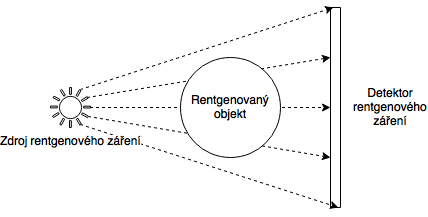
\includegraphics[width=\textwidth]{xray-scene}
\caption{Scéna pro pořizování rentgenových snímků.}
\label{fig:xray-scene}
\centering
\end{figure}

\subsection{Vznik rentgenového záření}
\label{sec:vznik-rentgenoveho-zareni}
Elektromagnetické záření, kterému se říká rentgenové záření vzniká buď při přechodu elektronů mezi vnitřními vrstvami těžších atomů -- charakteristické X-záření, nebo při dopadu a prudkém zabrzdění elektronů -- brzdné záření. \cite{AstroNuklFyzika-JadRadFyzika}

\subsubsection{Brzdné záření}
V případě, že se akcelerovaný elektron přiblíží k jádru atomu silné Coulombovy síly mezi jádrem atomu a letícím elektronem způsobí silné zbrzdění elektronu a změnu jeho trajektorie. Během zbrzdění rychle letícího elektronu  je jeho kinetická energie přeměňována na brzdné záření. \cite[str.~89]{Diagnostic-Radiology-Physics} Tento proces popisuje \cref{fig:bremsstrahlung-xray}.

\begin{figure}[bh]
\centering
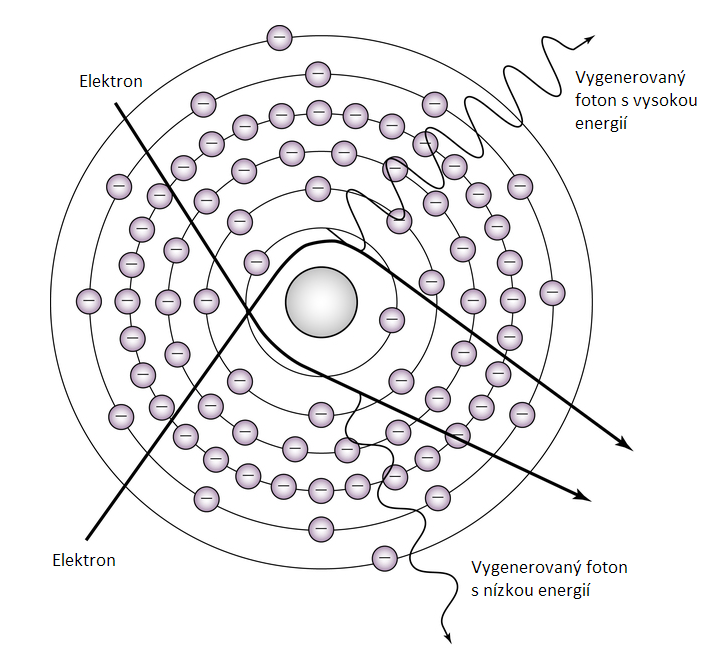
\includegraphics[width=0.75\textwidth]{bremsstrahlung-xray}
\caption{Vznik brzdného záření při interakci rychle se pohybujícího elektronu s atomem wolframu. \cite{the-xray-beam}}
\label{fig:bremsstrahlung-xray}
\end{figure}

Ideální spektrum brzdného záření lze popsat pomocí zjednodušeného modelu, který neuvažuje kvantovou mechaniku. Zjednodušený model uvažuje proud elektronů přibližující se k atomu. Uvážíme-li pole v okolí jádra atomu rozdělené na několik kruhových vrstev dle působících brzdných sil, generované brzdné záření brzděním proudu elektronů má spektrum, které odpovídá plochám těchto vrstev. Čím blíže je vrstva pole k jádru atomu, tím větší brzdnou sílou působí na letící elektron a tím větší je energie vygenerovaného fotonu. Zároveň čím je vrstva pole vzdálenější od jádra atomu, tím větší má plochu a tím více fotonů je schopna vygenerovat. Fotony generované ve vzdálenějších vrstvách mají nižší energii vzhledem k nižším brzdným silám působících na přibližující se elektrony. \cite[kap.~THE~X-RAY TUBE]{The-Physical-Principles-of-Medical-Imaging}

Ideální spektrum brzdného záření zjednodušeného modelu ukazuje \cref{fig:bremsstrahlung-xray-char}. Ze spektra je zřetelné, že největší energii, která se blíží kinetické energii elektronů má jen zlomek z celkového počtu generovaných fotonů (fotony generované elektrony, které byly zabrzděny ve vrstvě nejblíže jádru).

\begin{figure}[bh]
\centering
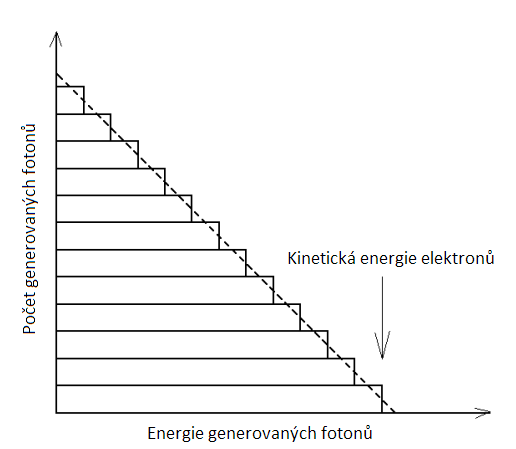
\includegraphics[width=0.75\textwidth]{bremsstrahlung-xray-char}
\caption{Ideální spektrum brzdného záření. \cite[str.~90]{Diagnostic-Radiology-Physics}}
\label{fig:bremsstrahlung-xray-char}
\end{figure}

\subsubsection{Charakteristické záření}
Charakteristické záření vzniká při přechodu atomového elektronu z vyšší vrstvy do nižší. Při přechodu elektron ztrácí energii, která je emitovaná jako foton charakteristického záření. Energie emitovaného fotonu odpovídá rozdílu energií vrstev mezi kterými elektron přechází. Spektrum charakteristického záření je monochromatické a odvíjí se od druhu atomu. Proces vzniku charakteristického záření popisuje \cref{fig:characteristic-xray}. \cite[str.~91]{Diagnostic-Radiology-Physics}

\begin{figure}[h]
\centering
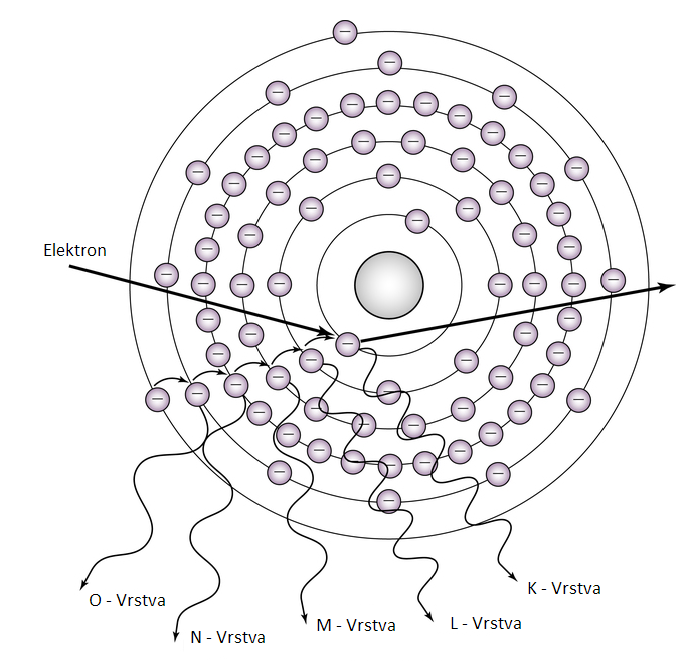
\includegraphics[width=0.75\textwidth]{characteristic-xray}
\caption{Vznik charakteristického záření v atomu wolframu při vyražení elektronu z K-Vrstvy elektronem s kinetickou energií vyšší, než vazební energie vyraženého elektronu. \cite{the-xray-beam}}
\label{fig:characteristic-xray}
\end{figure}

\subsection{Rentgenka}
Zdrojem rentgenového záření při pořizování rentgenových snímků je nejčastěji speciální vakuová elektronka (\cref{fig:xray-tube}), které je často nazývána jako rentgenka, rentgenová lampa či rentgenová trubice. \cite{AstroNuklFyzika-JadRadMetody} Rentgenku si lze představit, jako zařízení, které převádí energii elektronů na elektromagnetické záření s odpovídající energií. Expozice a spektrum záření může být řízena nastavením parametrů rentgenky jako jsou napětí (\SI{}{\kV}), proud (\SI{}{\mA}) a doba expozice (\SI{}{\s}). \cite[str.~93]{Diagnostic-Radiology-Physics}

\subsubsection{Principy fungování rentgenky}
Energie, která je přeměňována v rentgence na rentgenové záření a teplo je do rentgenky přiváděna proudem elektronů s potenciální energií odpovídající napětí na vysokonapěťovém zdroji (\SI{1}{\kV} odpovídá \SI{1}{\k\eV}). 
Během průchodu elektronu rentgenkou dochází k přeměně jeho potenciální energie na energii kinetickou, která je následně přeměněna na elektromagnetické záření a teplo. 

Kinetická energie elektronu při dopadu na anodu odpovídá napětí na vysokonapěťovám zdroji, tedy původní potenciální energii. Kinetická energie je přeměňována zbrzdění atomů při dopadu na anodu  při interakci s atomy materiálu na brzdné a charakteristické rentgenové záření. \cite[kap.~ELECTRON ENERGY]{The-Physical-Principles-of-Medical-Imaging}
Proud elektronu je emitován při žhavení katody se záporním napětí. Množství emitovaných elektronů může být řízeno změnou proudu žhavení, tedy změnou teploty žhaveného vlákna. \cite[str.~93]{Diagnostic-Radiology-Physics} 

\paragraph{Spektrum rentgenového záření rentgenky}
popisuje \cref{fig:xray-spectre}. Při dopadu elektronů na anodu vznikají dva typy rentgenového záření--brzdné a charakteristické, jejichž obecné principy byly popsány v kapitole \ref{sec:vznik-rentgenoveho-zareni}. Obrázek ukazuje celkem tři charakteristiky záření při napětí na elektrodách \SI{90}{\kV}:
\begin{enumerate}[label=(\alph*)]
\item Ideální spektrum brzdného brzdného záření--spektrum, které již bylo popsáno v obrázku \ref{fig:bremsstrahlung-xray-char}.
\item Generované spektrum--reálné spektrum skládající se z brzdného a charakteristického záření.
\item Filtrované spektrum--spektrum s útlumem dopovídajícím \SI{2.5}{\mm}Al.
\end{enumerate}

\begin{figure}[hb]
\centering
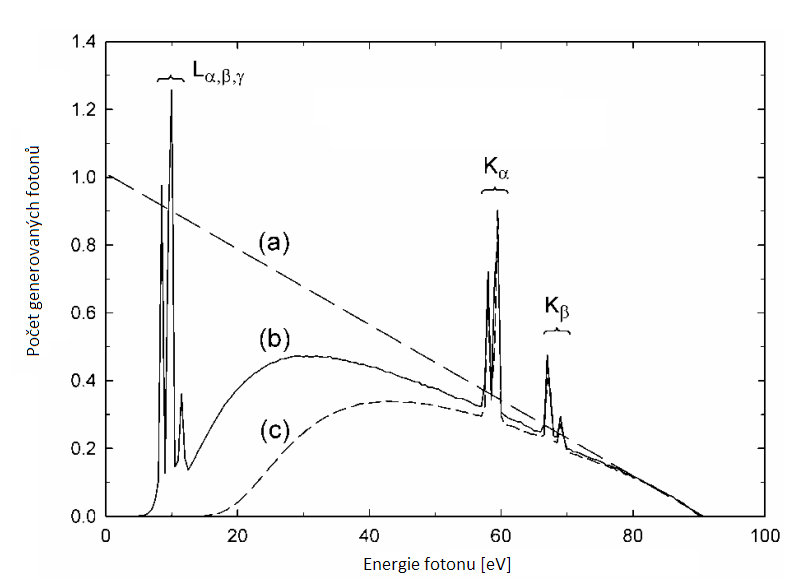
\includegraphics[width=\textwidth]{xray-spectre}
\caption{Rentgenka se zdroji proudu a napětí. \cite[str. 93]{Diagnostic-Radiology-Physics}}
\label{fig:xray-spectre}
\end{figure}

\subsubsection{Konstrukce rentgenky}
Z důvodu tepelného ohřevu anody po dopadu zrychlených elektronů a vysokého napětí na elektrodách musí být rentgenky oproti běžným elektronkám robustní konstrukce. Chlazení samotné anody je zajištěno její velikostí a také rotací  nebo aktivním chlazením. Rentgenky lze rozdělit kategorií podle způsobu využití a konstrukce \cite[kap. 3.2]{AstroNuklFyzika-JadRadMetody}:
\begin{itemize}
\item Rentgenky pro průmyslové ozařování a radioterapeutické použití - rentgenky s pevnou anodou, kde je chlazení zajištěno průtokem chladícího média. U toho typu rentgenek je častým požadavkem vysoká energie a intenzita záření. Naopak zde není potřebné zaměřování elektronů do téměř bodového ohniska. 
\item Rentgenky pro rentgenovou diagnostiku - rentgenky se soustředěním elektronů do ohniska. U tohoto typu rentgenek se využívá rotující anody proti nadměrnému přehřívání anody v místě ohniska.
\item Speciální rentgenky - rentgenky rozšířené o třetí elektrodu (drátěnou mřížku umístěnou mezi katodou a anodou v těsné blízkosti katody) sloužící k řízení proudu protékajícího anodou. Proud je řízen napětím, které je přivedeno na drátěnou mřížku.
\end{itemize}

Generované záření ještě před tím, než opustí rentgenku musí projít skrz různé materiály, které záření filtrují. Těmito materiály mohou být například samotná anoda, materiál trubice rentgenky, chladící medium apod. Úbytek záření při průchodu těmito materiály se uvádí jako útlum ekvivalentní k \SI{1}{\mm}Al--jednomu milimetru hliníku. Typická hodnota útlumu u běžných rentgenek bývá od \SI{0.5}{\mm}Al do \SI{1}{\mm}Al. 

\begin{figure}[hb]
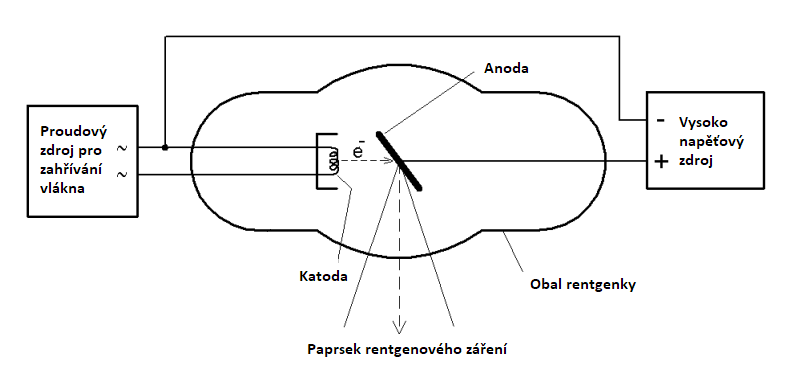
\includegraphics[width=\textwidth]{xray-tube}
\caption{Rentgenka se zdroji proudu a napětí. \cite[str. 93]{Diagnostic-Radiology-Physics}}
\label{fig:xray-tube}
\centering
\end{figure}

\paragraph{Anoda}
je součást rentgenky, kde je generováno rentgenové záření. Anoda bývá tvořena relativně velikým kusem železného materiálu, na který je přivedeno kladné napětí vysokonapěťového zdroje. Anoda jako taková plní v rentgence dvě funkce:
\begin{itemize}
\item Převod elektrické energie na rentgenové záření.
\item Odvod tepla, které vzniká během procesu generování rentgenového záření.
\end{itemize}
Jako vhodný materiál anody lze považovat materiál, který dokáže co největší podíl elektrické energie převést na záření, čili materiál, který má vysokou efektivitu převodu (jak již bylo zmíněno přebytečná energie je přeměňována na teplo). Efektivita převodu elektrické energie na záření závisí na atomovému číslu materiálu anody (Z) a kinetické energii dopadajícího elektronu na katodu.\cite{The-Physical-Principles-of-Medical-Imaging}

Nejvíce rentgenek využívá jako materiál anody wolfram s atomovým číslem 74. Wolfram je vhodný díky vysokému atomovému číslu a vysokému bodu tání. V některých případech je využíváno slitiny wolframu a rhenia, která je však využívána pouze jako povrchový materiál. Zbylá část anody anody poté bývá vyrobena z relativně lehkého materiálu, který má dobré tepelné vlastnosti. Těmito materiály mohou být například molybden nebo grafit. Výjimkou jsou anody rentgenek pro mamografii, kdy je využíváno molybdenu jako materiálu pro povrch anody.\cite{The-Physical-Principles-of-Medical-Imaging}

Anody lze dělit v závislosti na výkonu rentgenky (\cref{fig:anodes}). Pro aplikace, kdy není potřebná vysoká energie rentgenového záření je využíváno statických anod. Tato anoda se skládá z wolframu, který je usazen v měděném bloku, který slouží k odvádění tepla. Tento typ anod se využívá například dentistických nebo přenosných rentgenkách. Druhým typem anod jsou rotační anody. Anoda je připojená k rotoru asynchronního motoru, který je umístěn přímo ve vakuové trubici rentgenky. Vinutí statoru je naopak umístěno vně rentgenkové trubice. Samotná anoda má kruhový tvar v podobě terče se skosenými hranami na okrajích. Paprsek elektronů poté dopadá na zkosenou hranu, která je otáčena rotorem, tudíž je anoda tepelně namáhána rovnoměrně podél celého obvodu, což umožňuje generovat záření s vyšší energií. \cite[str.~98]{Diagnostic-Radiology-Physics}

\begin{figure}[hb]
\centering
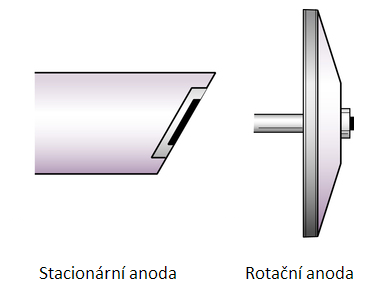
\includegraphics{anodes}
\caption{Rotační a stacionární anoda. \cite{the-xray-beam}}
\label{fig:anodes}
\end{figure}


\paragraph{Katoda}
je druhou elektrodou rentgenky, která má za úkol generování paprsku elektronů pomocí žhavícího vlákna (\cref{fig:cathode}). Katoda je připojena a záporné napětí vysokonapěťového zdroje a zároveň k střídavému zdroji proudu, který slouží k žhavení vlákna katody a tím i emitování elektronů.\cite[str.~93]{Diagnostic-Radiology-Physics} Velikost žhavícího vlákna ovlivňuje velikost ohniska paprsku elektronů na anodě. Čím větší je žhavící vlákno tím větší ohnisko je.

\begin{figure}[hb]
\centering
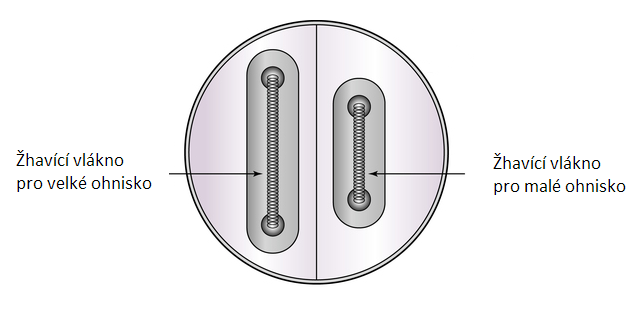
\includegraphics{cathode}
\caption{Katoda s dvěmi žhavícími vlákny. \cite{the-xray-beam}}
\label{fig:cathode}
\end{figure}

\subsection{Detekce rentgenového záření}
Rentgenové záření může být detekováno pomocí tzv. detektorů rentgenového záření. Tyto detektory lze dělit podle způsobu záznamu rentgenového záření na analogové a digitální. Analogové detektory využívají principu záznamu rentgenového záření v podobě snímku na film, kdežto digitální zaznamenávají snímky jako digitální snímek. Digitální detektory lze dělit dle toho, zda je snímek digitalizován přímo během procesu ozařování (\zkratka{zk:DR}) nebo až po procesu ozařování (\zkratka{zk:CR}). Systémy patřící do \zkratka{zk:DR} lze rozdělit dle toho, zda snímají přímo rentgenové záření nebo rentgenové záření převedené na světelné záření na \zkratka{zk:DR} s přímým a nepřímým převodem rentgenového záření. V případě digitálních detektorů je často zmiňována velikost pixelů. Touto velikostí je myšlena plocha snímače rentgenové nebo světelného záření detektoru, který dopovídá jednomu pixelu.

\subsubsection{Parametry detektorů}
\paragraph{Velikost pixelu, velikost detektoru a rozlišení}
jsou jedněmi ze základních parametrů digitálních detektorů. Velikost pixelů, respektive velikost snímací plochy snímače odpovídající pixelu a vzdálenost mezi nimi ovlivňují především prostorové rozlišení detektoru. \cite[str.~682]{Advances-in-Digital-Radiography} Celková velikost detektoru poté ovlivňuje jak velkou scénu lze snímat (flat-panel detektory), případně jaký způsobem je scéna snímána (snímání pohybujícího se rentgenovaného předmětu nebo scény pomocí řádkového CCD detektoru např. na výrobní lince). Rozlišení digitálních detektorů odpovídá počtu pixelů/snímačů a je udáváno v počtech pixelů na šířku a výšku.

\paragraph{Prostorové rozlišení}
představuje minimální vzdálenost mezi dvěma kontrastními objekty, při které lze tyto dva objekty pomocí detektoru od sebe rozlišit. \cite[str.~682]{Advances-in-Digital-Radiography} Jinými slovy je to vzdálenost mezi dvěma objekty na rentgenovém snímku, při kterém nám tyto dva objekty nesplývají v jeden. Jak již bylo zmíněno, maximální prostorové rozlišení digitálních detektorů vychází z minimální velikosti pixelů těchto detektorů. Vezmeme-li v potaz Nyquistův teorém o vzorkovací frekvenci, maximální dosažitelné rozlišení v případě, že má pixel velikost $a$ je nižší než $a/2$. 

Mimo minimální velikosti pixelů prostorové rozlišení ovlivňuje také rozptyl uvnitř detektorů. Například selenové polovodičové detektory s přímým převodem mají lepší prostorové rozlišení než detektory s nepřímým převodem s nestrukturovanou scintilační vrstvou.

\paragraph{Modulační přenosová funkce -- Modulation Transfer Function (MTF)}
úzce souvisí s prostorovým rozlišením detektoru. \zk{zk:MTF} jako jednotka je vhodná pro určení pravého nebo efektivního rozlišení detektoru, protože zahrnuje míru rozostření a změny kontrastu v v určitém rozsahu prostorových frekvencí.\zk{zk:MTF} lze definovat jako podíl kontrastu výstupního signálu detektoru ku kontrastu vstupního signálu detektoru. \cite{Modulacni-Prenosova-Funkce} Jinými slovy \zk{zk:MTF} říká, jak se  přemění kontrast vstupního signálu detektoru pro určitou prostorovou frekvenci vstupního signálu na kontrast výstupního signálu. \cite[str.~682]{Advances-in-Digital-Radiography} Prostorová frekvence vstupního signálu je uváděna v cyklech na \SI{}{\mm}.

\paragraph{Dynamický rozsah}
detektoru vyjadřuje odezvu výstupu detektoru na jeho vstup. Dynamický rozsah je popsán funkcí dávky rentgenového záření jejíž výstupem jsou hodnoty v rozsahu od minimální do maximální možné hodnoty výstupu detektoru. Například v případě filmových systémů je tento rozsah poměrně malý, tudíž se může stát, že nesprávně zvolenou expoziční dobou dochází k přeexponování snímku. Naopak u digitálních detektorů je dynamický rozsah detektoru poměrně vysoký, čímž riziko přeexponování snímku klesá, ale naopak například v lékařské praxi může docházet k vystavování pacienta zbytečně velké dávce rentgenového záření. Závislosti výstupů filmových a obecných digitálních detektorů na dávce rentgenového záření popisuje \cref{fig:dynamic-range}. \cite[str.~682]{Advances-in-Digital-Radiography}

\begin{figure}[ht]
\centering
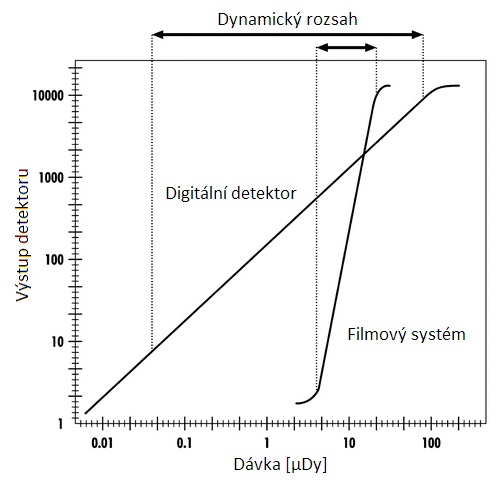
\includegraphics{dynamic-range}
\caption{Závislost výstupu detektorů na dávce rentgenového záření. \cite[str.~682]{Advances-in-Digital-Radiography}}
\label{fig:dynamic-range}
\end{figure}

\paragraph{Detekční kvantová účinnost -- Detective Quantim Efficiency (DQE)}
určuje účinnost detektoru při převodu energie fotonu rentgenového záření na výstupní signál. \zk{zk:DQE} lze popsat jako poměr poměru signál-šum -- signal-to-noise ratio (SNR) výstupního signálu ku SNR vstupního signálu. SNR výstupního a vstupního signálu je funkce závislá na prostorové frekvenci. \zk{zk:SNR} a tím i \zk{zk:DQE} jsou závislé na frekvenci, \zk{zk:MTF} a materiálu detektoru. 

Čím vyšší hodnota \zk{zk:DQE} je, tím menší dávka rentgenového záření je potřeba k získání snímku o stejné kvalitě oproti detektoru s nižší hodnotou \zk{zk:DQE}. Tato závislost lze také vyjádřit tak, že při stálé době expozice detektor s vyšší \zk{zk:DQE} detekuje kvalitnější snímek oproti detektoru s nižší hodnotou \zk{zk:DQE}. Hodnota \zk{zk:DQE} ideálního detektoru je hodnota 1. V tomto případě by byl detektor schopen přeměnit veškerou energii rentgenového záření na obrazovou informaci.

\subsubsection{Filmové systémy}
Pro získávání snímků pomocí filmu je využíváno filmových systému. Tento systém využívá filmu, který je citlivý na světelné záření. Pro získání rentgenového snímku je třeba vložit film do rentgenového zařízení a poté film vyvolat. Film bývá vložen do plastové kazety, uvnitř kterých je fosforová vrstva, která přeměňuje rentgenové záření na světelné záření, které lze detekovat filmem vloženým do kazety. Výhodou filmových systémů je, že film jako takový má vysokou citlivost a zároveň se při detekci na rozdíl od digitálních systémů neztrácí žádná viditelná informace. \cite[str.~155]{Diagnostic-Radiology-Physics} Filmové systémy jsou využívány jak ve zdravotnictví, tak v průmyslu, nicméně jejich využití je spíše na ústupu. Vzhledem k povaze této práce se jimi práce nebude více zabývat.

\subsubsection{Digitální systémy}
Čím dál častěji filmové systémy nahrazují systémy digitální. tyto systémy lze rozdělit do dvou kategorií na systémy pro nepřímou radiografii -- Computed Radiography (\zk{zk:CR}) a přímou radiografii -- Direct Radiography  (\zk{zk:DR}). \zk{zk:CR} vychází z klasických filmových systému u kterých je místo filmu využíváno speciálních fosforových fólií. Proces digitalizace je pak prováděn ve speciálním zařízení.
\zk{zk:DR} na rozdíl od \zk{zk:CR} převádí záření na digitální snímek přímo, nicméně samotný proces převodu může být přímý (záření je převáděno snímači na elektrickou veličinu) nebo nepřímý (záření je nejprve převedeno na světelné záření, které je poté převáděno na elektrickou veličinu). \cite[str.~676]{Advances-in-Digital-Radiography}

\paragraph{Nepřímá radiografie (\zk{zk:CR})}
využívá technologie, která je velice podobná filmovým systémům. Paměťové fólie jsou tvořeny citlivou vrstvou tvořenou fosforovými krystaly. \cite[str.~676]{Advances-in-Digital-Radiography}. 

Proces ukládání informace a její digitalizaci popisuje \cref{fig:cr}. Energie dopadajícího záření je absorbována a dočasně (řádově několik hodin) uložena v paměťové fólii přechodem elektronů atomů fosforových krystalů do vyšších energických hladin (metastabilních). Digitalizace uložené energie ve fólii poté probíhá v zařízení, které dokáže pomocí laserového paprsku uvolňovat elektrony z metastabilních hladin do vodivostního pásu. Při uvolňování elektronů dochází k emitování světelného záření, které je poté možné měřit fotonásobičem připojeným na AD převodník. \cite[str.~677]{Advances-in-Digital-Radiography}. Výhodou tohoto systému je snadná integrace do stávajících filmových systémů. Nevýhodou může být vysoká časová náročnost vyvolávání snímků, nízké prostorové rozlišení. \cite[str~209]{Diagnostic-Radiology}

\begin{figure}[ht]
\centering
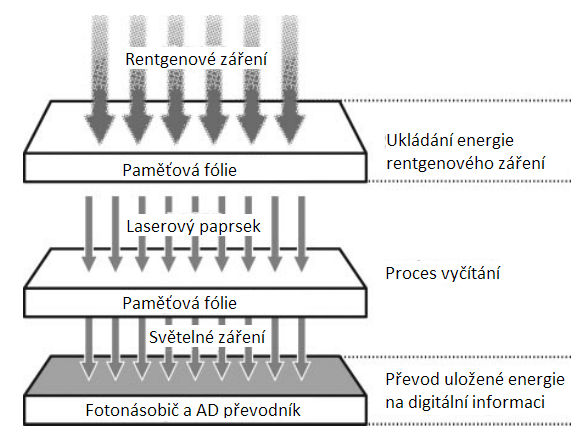
\includegraphics{cr}
\caption{Proces získání digitálního snímku při nepřímé radiografii. \cite[str.~677]{Advances-in-Digital-Radiography}}
\label{fig:cr}
\end{figure}

\paragraph{Přímá radiografie (\zk{zk:DR})}
\zk{zk:DR} je možné dále dělit podle způsobu převodu rentgenového řazení na \zk{zk:DR} s přímým  převodem a \zk{zk:DR} s nepřímým převodem. Při přímém převodu je rentgenové záření snímáno přímo, naopak při nepřímém převodu je záření převáděno zpravidla pomocí scintilační vrstvy na záření světelné, které je poté snímáno fotocitlivými snímači. Rozdíl mezi přímým a nepřímým převodem rentgenového záření popisuje obrázek \cref{fig:direct-indirect-tft}.

\begin{figure}[ht]
\centering
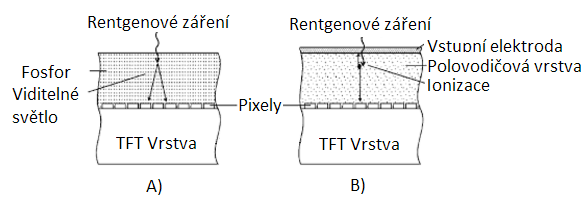
\includegraphics{direct-indirect-tft}
\caption{Polovodičový TFT detektor s nepřímým (A) a přímým (B) převodem rentgenového záření \cite[str.~511]{Radiation-Detection-and-Measurement}}
\label{fig:direct-indirect-tft}
\end{figure}

\paragraph{DR s přímým převodem}
využívají polovodičové vrstvy ze selenu (Se), který dokáže převádět fotony rentgneového záření na elektrickou energii. \zk{zk:DR} systémy s přímým převodem mohou využívat buď selenové foto-válce s AD převodníkem nebo selenové polovodičové vrstvy spojené s vrstvou tenkovrstvých tranzistorů -- Thin Film Tranzistors (\zk{zk:TFT}). \cite[str.~678]{Advances-in-Digital-Radiography} Výhodou těchto systémů je především vysoké prostorové rozlišení. Díky nízkému atomovéu číslu selenu je u těchto detektorů poměrně nízká absorpce rentgenového záření. Díky tomuto faktu je systémů s přímým převode využíváno spíše v mamografii. \cite[str~210]{Diagnostic-Radiology}

Systémy, které využívají foto-válců otáčí samotným válcem, na který dopadá rentgenové záření, které se přeměňuje na náboj na povrchu válce. Náboj na povrchu otáčejícího se válce je poté vyčítán pomocí AD převodníku. \cite[str.~677]{Advances-in-Digital-Radiography}. Tento princip je založen na stejném principu jako foto válec laserových tiskáren.
 
Na podobné principu pracují systémy s vrstvou \zk{zk:TFT} (\cref{fig:direct-tft}). Matice \zk{zk:TFT} ukládá generovaných náboj do paměťových kondenzátorů, jejichž napětí může být vyčítáno AD převodníkem. Takovýto detektor se skládá z elektrody na kterou je přivedeno vysoké kladné napětí, polovodičové vrstvy selenu a vrstvy \zk{zk:TFT} kondenzátory pro ukládání náboje generovaného rentgenovým záření. Rentgenové záření generuje v selenové vrstvě elektrony a díry. Díky tomu vzniká v polovodiči náboj, který je přímo úměrný rentgenovému rentgenovému záření. Tento náboj je poté díky silnému elektrickému poli odváděn do kondenzátorů v \zk{zk:TFT} vrstvě. Napětí kondenzátoru může být poté vyčteno přivedení záporného napětí na gate příslušného tranzistoru.

\begin{figure}[ht]
\centering
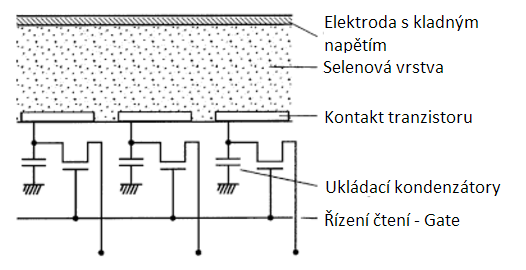
\includegraphics{direct-tft}
\caption{Princip polovodičového TFT detektoru s přímým převodem rentgenového záření \cite[str.~511]{Radiation-Detection-and-Measurement}}
\label{fig:direct-tft}
\end{figure}

\paragraph{DR s nepřímým převodem}
využívá scintilační vrstvy k převodu rentgenového záření na světelné záření, které je poté snímáno dalšími vrstvami. Scintilační vrstvy můžou být jak strukturované, tak nestrukturované. V případě nestrukturované scintilační vrstvy generované světelné záření přirozeně dopadá na přilehlé snímače světelného záření, které odpovídají jednotlivým pixelům. Naopak v případě strukturované scintilační vrstvy světelné záření díky speciální struktuře vrstvy dopadá pouze na jeden snímač světelného záření. Díky tomu je zajištěno lepší prostorové rozlišení detektoru. Rozdíly mezi strukturovanou a nestrukturovanou scintilační vrstvou popisuje \cref{fig:structured-unstructured-scintillator}.

\begin{figure}[ht]
\centering
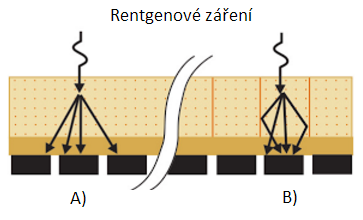
\includegraphics{structured-unstructured-scintillator}
\caption{Rozdíl mezi nesturkturovanou (A) a strukturovanou (B) scintilační vrstvou TFT detektoru s nepřímým převodem. \cite[str~210]{Diagnostic-Radiology}}
\label{fig:structured-unstructured-scintillator}
\end{figure}

V případě, že je jako detekční vrstva využíváno \zk{zk:TFT} matice, musí být pod scintilační vrstvu přidána vrstva detekující světelné záření. Taková vrstva je nejčastěji tvořena foto-diodovým polem. Elektrická energie generována foto-diodovým polem je poté ukládána pomocí kondenzátorů \zk{zk:TFT} matice a následně  čtena AD převodníkem.

Detekční vrstva může být také realizována pomocí \zkratka{zk:CCD}. V tomto případě je pomocí \zk{zk:CCD} detektorů přímo detekováno viditelné světlo, které je generováno v scintilační vrstvě. Díky poměrně malé velikosti \zk{zk:CCD} snímačů je nutné snímače kombinovat do matic, případně využívat čoček.

\section{Metody předzpracování rentgenových snímků}

\subsection{Reprezentace digitálního snímku}
Pořízený digitální snímek může být reprezentován pomocí signálu v prostorové nebo frekvenční oblasti. Způsob reprezentace pořízeného obrázku se odvíjí především od způsobu jeho pořizování. V případě digitální radiografie jsou snímky pořizovány v prostorové oblasti. Snímky ve frekvenční oblasti lze například nalézt u magnetické rezonance -- Magnetic Resonance Inspection (MRI).

\paragraph{Prostorová oblast}
digitálních snímků je reprezentována pomocí matice o velikosti $M \times N$, kde $M$ je počet řádků a $N$ počet sloupců. Jednotlivé prvky matice se nazývají pixely. Počet sloupců a řádků určuje rozlišení snímku a je udáváno jako $M \times N$ nebo jako výsledek jejich součinu, čili absolutní počet pixelů -- například rozlišení $1024 \times 1024$ lze zapsat jako \num{1048576} pixelů.  Pixely mohou nabývat hodnot od 0 do $2^{n}$, kde číslo $n$ je nazýváno jako bitová hloubka snímků. V případě digitálních rentgenových snímků bývá datová hloubka nejčastěji 10, 12 nebo 16 bitů, nicméně hodnota bývá zpravidla ukládána ve 2 bytech, tudíž v případě bitové hloubky 10 nebo 12 bitů zůstávají vyšší bity nulové.

Digitální snímek v prostorového oblasti se skládá z kanálů, které jsou reprezentovány pomocí matic o stejném počtu řádků a sloupců, jako má výsledný digitální snímek. Počet kanálů a to, co reprezentují je určeno barevným modelem. Například jedním z nejznámějších barevných modelů je model RGB, který definuje 3 barevné kanály: červený (RED), zelený (GREEN) a modrý (BLUE). Každý kanál reprezentuje intenzitu jedné z barev a jejich sečtením vzniká výsledný snímek. Vzhledem k způsobu pořizování rentgenových snímků, mají snímky pouze jeden kanál, který zpravidla bývá interpretován pomocí stupňů šedi -- grayscale.

\paragraph{Frekvenční oblast}
digitální snímků reprezentuje frekvence obsažené v obrázku. Frekvence signálu digitálního snímku odpovídá počtu cyklů na jeden pixel. Například pokud snímek obsahuje řádek, který se skládá z periodicky se opakující dvojice černého a bílého pixelu, digitální snímek bude obsahovat signál o frekvenci \SI{1/2}{\hertz}. 

Vzhledem k tomu, že ve většině případů je pořízený snímek v prostorové oblasti musí být snímek do frekvenční oblasti převeden. V případě digitálních snímků bývá pro převod nejčastěji využíváno diskrétní Fourierovy transformace (DFT). Pro zpětný převod je poté využíváno zpětné DFT. DFT je definována jako:
\begin{equation}
\label{eq:dft}
F(u,v)=\sum_{x=0}^{M-1} \sum_{y=0}^{N-1} f(x,y) e^{\frac{-j2\pi ux}{M} - \frac{j2\pi vy}{N}}
\end{equation}
a zpětnou DFT jako:
\begin{equation}
f(x,y)=\frac{1}{MN}\sum_{u=0}^{M-1}\sum_{v=0}^{N-1}F(u,v)e^{\frac{j2\pi ux}{M}+\frac{j2\pi vy}{N}},
\end{equation}
kde $f(n,m)$ představuje konkrétní pixel obrázku v prostorové oblasti s indexem $n$ a $m$, $N$ a $M$ jsou rozměry velikost snímku, $F(k,l)$ je reprezentace snímku ve frekvenční oblasti pro různé frekvence reprezentované pomocí $k$ a $l$. Velikost $k$ a $l$ se pohybuje v rozsahu od 0 do $M-1$ a od 0 do $N-1$
, přičemž $F(0,0)$ udává velikost stejnosměrné složky obrázku a $F(M-1,N-1)$ udává velikost složky s nejvyšší možnou frekvencí. Normalizační člen zpětné DFT $\frac{1}{MN}$ může být přesunuta do rovnice \ref{eq:dft}, kdy pro $F(0,0)$ je poté stejnosměrná složka rovna průměrné hodnotě pixelů snímku.

\subsection{Metody předzpracování rentgenových snímků}
Operace prováděné při předzpracování digitálních RTG snímků lze dle Baxese \cite{baxes} a Gonzáleze \cite{Gonzalez} rozdělit do pěti základních kategorií. Tyto kategorie zahrnují:
\begin{itemize}
\item Obnovení -- obnovení poškozených snímků například kompresí, rozmazáním či ztrátou dat.
\item Analýzu -- operace zahrnující segmentaci, klasifikaci apod. 
\item Syntézu -- sloučení více snímků pro získání více informací. Sloučením může vzniknout například nový snímek nebo 3D model v případě \zkratka{zk:CT}.
\item Zvýšení kvality -- operace sloužící pro zvýšení kvality za účelem zvýšení diagnostické hodnoty snímku. Nejčastěji se jedná o zvýraznění hran, úpravu kontrastu apod.
\item Kompresi -- snížení velikosti snímků.
\end{itemize}

V případě digitálních rentgenových snímků a metod jejich předzpracování se můžeme setkat s operacemi ze všech kategorií. V případě operací pro obnovení se nejčastěji setkáváme s odstraněním šumu který vzniká díky nehomogenitě generovaného rentgenového záření. Operace pro analýzu zahrnují především segmentaci obrazu a klasifikaci. V případě operací pro zvyšování kvality je v radiologii využíváno především zvýrazňování hran, úpravy kontrastu a dynamického rozsahu. Kompresní operace jsou využívány především při ukládání a archivaci digitálních snímků, kdy je kladen důraz na snížení velikosti digitálních snímků při zachování jejich dostatečné kvality.

\subsubsection{Odstranění šumu}
Filtrováním digitálních rentgenových snímků se rozumí provádění operací za účelem zvýšení jejich kvality, především z hlediska rozlišení, kontrastu a šumu. V případě filtrování v prostorové oblasti jsou operace prováděny postupně na jeden nebo skupinu pixelů.
\paragraph{Průměrování}
je jedním z nejjednodušších filtrů. Funguje na principu nahrazení hodnoty pixelu hodnotou průměru jeho okolí o velikosti $N$. Díky nahrazení hodnoty pixelu průměrem jeho okolí dochází k filtrování složek s vysokou frekvencí ve frekvenční oblasti. Vliv filtru a změny velikosti jeho okolí ukazuje \cref{fig:mean-filter}. Z obrázku je zřejmé, že filtr filtruje vysokofrekvenční složky -- tmavá linka ve spodní části obrázku a čáry na obloze. Matematicky lze průměrovací filtr vyjádřit pomocí konvoluce následovně:

\begin{equation}
\label{eq:mean1}
I_{filtered} = I \ast K
\end{equation}
\begin{equation}
\label{eq:mean2}
K = \frac{1}{N^{2}}\begin{bmatrix}
 &1  &1 &\dots  &1 \\ 
 &1  &1 &\dots  &1 \\ 
 &\vdots  &\vdots &\ddots  &\vdots \\ 
 &1  &1 &\dots  &1 
\end{bmatrix},
\end{equation}
kde $N$ určuje velikost okolí -- velikost konvoluční matice $N\times N$, $I$ filtrovaný snímek a $I_{filtered}$ snímek po aplikaci filtru.

\begin{figure}[h]
\centering
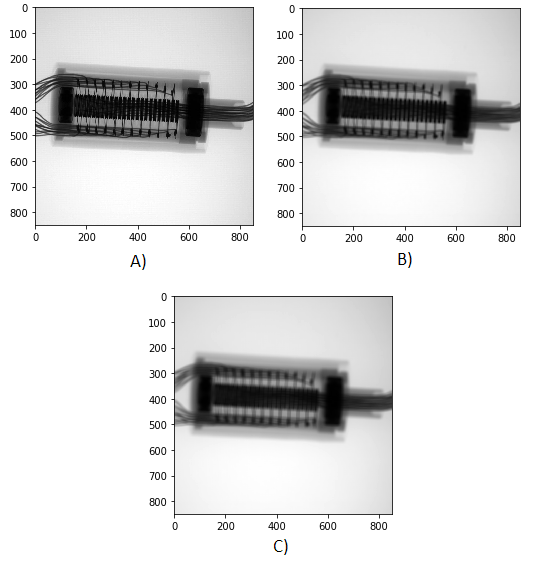
\includegraphics{mean-filter}
\caption{Původní snímek (A) a snímky na které je aplikován průměrovací filtr s okolím $\protect N=10$ (B) a okolím $\protect N=15$ (C).}
\label{fig:mean-filter}
\end{figure}

Ve vztahu k radiologii průměrovací filtr dokáže vyhladit snímek díky odstranění šumu s vysokou frekvencí. Mimo odstranění šumu je průměrovací filtr využíván před dalšími kroky předzpracování digitálních rentgenových snímků. \cite{Diagnostic-Radiology-Physics}

\paragraph{Gaussův filtr}
lze stejně jako průměrovací filtr definovat pomocí konvoluce a stejně jako průměrovací filtr se chová jako dolnopropustní filtr -- filtruje vysokofrekvenční složky. V případě Gaussova filtru však konvoluční matice nezajišťuje průměrování, ale je vygenerována na základě aproximace Gaussova rozložení dle rovnice \cite[str.~139]{Image-Processing-Analysis-and-Machine-Vision}:

\begin{equation}
\label{eq:gaussian1}
G(x,y)=e^{\frac{-(x^2+y^2)}{2\sigma^2}},
\end{equation}
kde $x$ a $y$ jsou souřadnice a $\sigma$ směrodatná odchylka. Často bývá rovnice \ref{eq:gaussian1} rozšiřována o normalizační členy:
\begin{equation}
\label{eq:gaussian2}
G(x,y)= \frac{1}{2\pi\sigma^2} e^{\frac{-(x^2+y^2)}{2\sigma^2}} 
\end{equation}
\begin{equation}
\label{eq:gaussian3}
G(x,y)= \frac{1}{\sqrt{2\pi}\sigma} e^{\frac{-(x^2+y^2)}{2\sigma^2}}
\end{equation}

Vzhledem k tomu, že normální rozložení lze definovat pro všechna reálná čísla, výsledná matice by byla nekonečně veliká, proto se v praxi často velikost matice omezuje tak, aby matice obsahovala všechny hodnoty normálního rozložení v intervalu $<-3\sigma, 3\sigma>$. Aplikaci Gaussova filtru na reálný snímek popisuje \cref{fig:gaussian-filter}. Stejně jako u průměrovacího filtru je z obrázku zřejmá dolnopropustní charakteristika Gaussova filtru.

\begin{figure}[h]
\centering
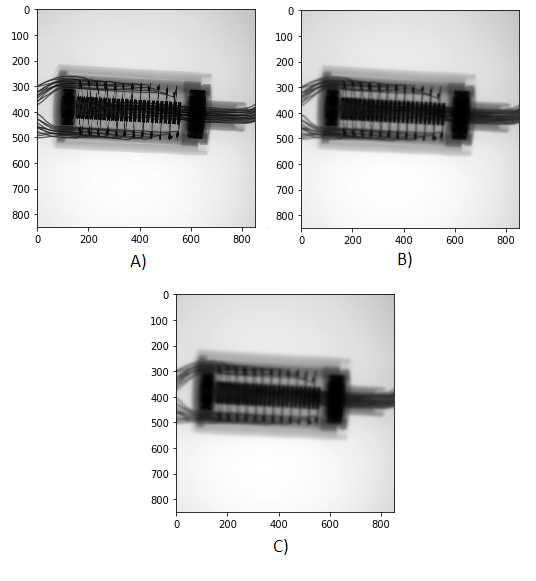
\includegraphics{gaussian-filter}
\caption{Původní snímek (A) a snímky na které je aplikován Gaussův filtr s parametrem $\protect\sigma=3$ (B) a $\protect\sigma=5$ (C).}
\label{fig:gaussian-filter}
\end{figure}

\paragraph{Mediánový filtr} nahrazuje každý pixel snímku mediánem hodnot v okolí pixelu $N \times N$. Medián hodnot jako takový je nelineární operace, proto ho není možné reprezentovat pomocí konvoluce jako v případě průměrovacího a Gaussova filtru. Mediánový filtr je využívám především k odstranění impulsového šumu. Jinými slovy šumu, který způsobuje, že některé izolované pixely mají velmi nízkou nebo naopak vysokou hodnotu oproti svému okolí. Nevýhodou tohoto filtru je, že může odstranit pro nás důležité informace, jako tenké hrany apod. Filtraci snímku, který je uměle zašuměný náhodným šumem typu "salt \and pepper" $20\%$ pokrytím snímku, ukazuje \cref{fig:median-filter}.

\begin{figure}[h]
\centering
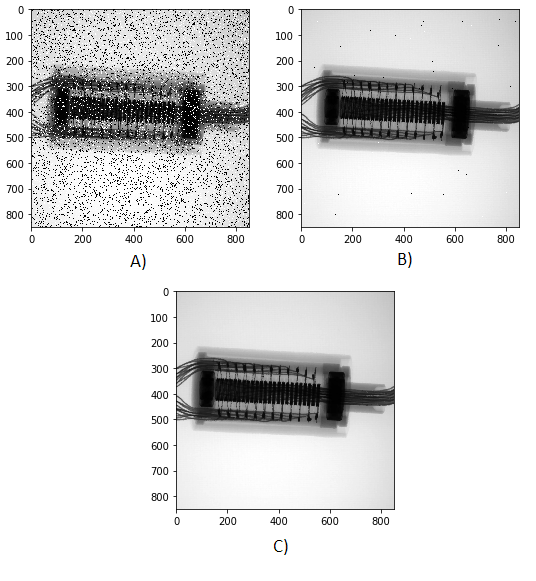
\includegraphics{median-filter}
\caption{Snímek zašumělý pomocí náhodného šumu "salt \and pepper" (A) a snímky na které je aplikován mediánový filtr s parametrem okolí $\protect N=3$ (B) a $\protect N=5$ (C).}
\label{fig:median-filter}
\end{figure}



%% Vložení souboru 'text/vysledky' s popisem vysledků práce
\chapter{Výsledky studentské práce}

Praktická část a výsledky studenstké práce vhodně rozdělené do částí.

\section{Programové řešení}
Lorem ipsum dolor sit amet, consectetuer adipiscing elit. Nulla pulvinar eleifend sem. Integer in sapien. Etiam sapien elit, consequat eget, tristique non, venenatis quis, ante. In laoreet, magna id viverra tincidunt, sem odio bibendum justo, vel imperdiet sapien wisi sed libero. Aliquam in lorem sit amet leo accumsan lacinia. Cum sociis natoque penatibus et magnis dis parturient montes, nascetur ridiculus mus. Duis sapien nunc, commodo et, interdum suscipit, sollicitudin et, dolor. Suspendisse sagittis ultrices augue. Nullam lectus justo, vulputate eget mollis sed, tempor sed magna. In convallis. Praesent id justo in neque elementum ultrices. Neque porro quisquam est, qui dolorem ipsum quia dolor sit amet, consectetur, adipisci velit, sed quia non numquam eius modi tempora incidunt ut labore et dolore magnam aliquam quaerat voluptatem. Phasellus enim erat, vestibulum vel, aliquam a, posuere eu, velit. Aliquam erat volutpat. Nullam faucibus mi quis velit \cite{sr02/2009}.

Aliquam erat volutpat. Quisque porta. Integer imperdiet lectus quis justo. Nullam justo enim, consectetuer nec, ullamcorper ac, vestibulum in, elit. Nullam faucibus mi quis velit. Fusce tellus. Fusce consectetuer risus a nunc. Cras pede libero, dapibus nec, pretium sit amet, tempor quis. Morbi imperdiet, mauris ac auctor dictum, nisl ligula egestas nulla, et sollicitudin sem purus in lacus
\cite{CSN_ISO_690-2011,CSN_ISO_7144-1997,CSN_ISO_31-11}.
Mauris elementum mauris vitae tortor. Neque porro quisquam est, qui dolorem ipsum quia dolor sit amet, consectetur, adipisci velit, sed quia non numquam eius modi tempora incidunt ut labore et dolore magnam aliquam quaerat voluptatem. Quisque porta. Integer vulputate sem a nibh rutrum consequat. Nulla pulvinar eleifend sem. Praesent id justo in neque elementum ultrices \cite{BiernatovaSkupa2011:CSNISO690komentar}.

\section{Výsledky měření}
Fusce tellus odio, dapibus id fermentum quis, suscipit id erat. Fusce tellus. Morbi scelerisque luctus velit. In laoreet, magna id viverra tincidunt, sem odio bibendum justo, vel imperdiet sapien wisi sed libero. Quisque porta. Fusce suscipit libero eget elit. Nulla non lectus sed nisl molestie malesuada. Phasellus faucibus molestie nisl. Integer vulputate sem a nibh rutrum consequat. Proin mattis lacinia justo. Phasellus et lorem id felis nonummy placerat. Etiam ligula pede, sagittis quis, interdum ultricies, scelerisque eu. Cras elementum. Aenean placerat. Donec ipsum massa, ullamcorper in, auctor et, scelerisque sed, est. Aliquam ante. Integer imperdiet lectus quis justo. Vivamus ac leo pretium faucibus. Nullam faucibus mi quis velit.

Etiam quis quam. Neque porro quisquam est, qui dolorem ipsum quia dolor sit amet, consectetur, adipisci velit, sed quia non numquam eius modi tempora incidunt ut labore et dolore magnam aliquam quaerat voluptatem. Aliquam erat volutpat. Lorem ipsum dolor sit amet, consectetuer adipiscing elit \cite{sr02/2009,pravidla}. Nunc auctor. Neque porro quisquam est, qui dolorem ipsum quia dolor sit amet, consectetur, adipisci velit, sed quia non numquam eius modi tempora incidunt ut labore et dolore magnam aliquam quaerat voluptatem. Maecenas lorem. Maecenas libero. In laoreet, magna id viverra tincidunt, sem odio bibendum justo, vel imperdiet sapien wisi sed libero. Nullam rhoncus aliquam metus.

Integer rutrum, orci vestibulum ullamcorper ultricies, lacus quam ultricies odio, vitae placerat pede sem sit amet enim. Ut enim ad minim veniam, quis nostrud exercitation ullamco laboris nisi ut aliquip ex ea commodo consequat. Fusce tellus odio, dapibus id fermentum quis, suscipit id erat. Nullam eget nisl. Nunc auctor. Etiam dui sem, fermentum vitae, sagittis id, malesuada in, quam. Fusce dui leo, imperdiet in, aliquam sit amet, feugiat eu, orci. Curabitur vitae diam non enim vestibulum interdum. Aliquam erat volutpat. Pellentesque sapien. Phasellus enim erat, vestibulum vel, aliquam a, posuere eu, velit.

Fusce dui leo, imperdiet in, aliquam sit amet, feugiat eu, orci. Maecenas aliquet accumsan leo. Aliquam ornare wisi eu metus. Cum sociis natoque penatibus et magnis dis parturient montes, nascetur ridiculus mus. Aliquam erat volutpat. Donec iaculis gravida nulla. Sed elit dui, pellentesque a, faucibus vel, interdum nec, diam. Temporibus autem quibusdam et aut officiis debitis aut rerum necessitatibus saepe eveniet ut et voluptates repudiandae sint et molestiae non recusandae. Nulla non arcu lacinia neque faucibus fringilla. Phasellus enim erat, vestibulum vel, aliquam a, posuere eu, velit. Praesent vitae arcu tempor neque lacinia pretium
\cite{Walter1999,Svacina1999IEEE,RajmicSysel2002}.

Fusce suscipit libero eget elit. Integer vulputate sem a nibh rutrum consequat. Aliquam erat volutpat. Etiam neque. Nulla turpis magna, cursus sit amet, suscipit a, interdum id, felis. Nullam rhoncus aliquam metus. Etiam dui sem, fermentum vitae, sagittis id, malesuada in, quam. Nunc auctor. Nunc dapibus tortor vel mi dapibus sollicitudin. Praesent in mauris eu tortor porttitor accumsan. Nulla non arcu lacinia neque faucibus fringilla. Nullam lectus justo, vulputate eget mollis sed, tempor sed magna. Maecenas lorem. Aenean placerat. Donec vitae arcu. Maecenas lorem. Donec iaculis gravida nulla. Nulla non lectus sed nisl molestie malesuada.

Duis pulvinar. Nulla est. Duis condimentum augue id magna semper rutrum. Integer pellentesque quam vel velit. Aliquam ante. Nulla quis diam. Proin mattis lacinia justo. Aenean fermentum risus id tortor. Nunc auctor. Nullam justo enim, consectetuer nec, ullamcorper ac, vestibulum in, elit. In dapibus augue non sapien. Etiam bibendum elit eget erat. In sem justo, commodo ut, suscipit at, pharetra vitae, orci. Maecenas libero.

Nulla non lectus sed nisl molestie malesuada. Donec vitae arcu. Aenean fermentum risus id tortor. Praesent in mauris eu tortor porttitor accumsan. Nulla pulvinar eleifend sem. Duis viverra diam non justo. Integer imperdiet lectus quis justo. Pellentesque habitant morbi tristique senectus et netus et malesuada fames ac turpis egestas. In rutrum. Excepteur sint occaecat cupidatat non proident, sunt in culpa qui officia deserunt mollit anim id est laborum. Nulla non lectus sed nisl molestie malesuada. Aliquam erat volutpat. Mauris tincidunt sem sed arcu. Duis bibendum, lectus ut viverra rhoncus, dolor nunc faucibus libero, eget facilisis enim ipsum id lacus. Fusce tellus odio, dapibus id fermentum quis, suscipit id erat. In enim a arcu imperdiet malesuada. Nulla non lectus sed nisl molestie malesuada. Proin mattis lacinia justo.


%Pellentesque pretium lectus id turpis. Nemo enim ipsam voluptatem quia voluptas sit aspernatur aut odit aut fugit, sed quia consequuntur magni dolores eos qui ratione voluptatem sequi nesciunt. Curabitur ligula sapien, pulvinar a vestibulum quis, facilisis vel sapien. Praesent dapibus. Sed elit dui, pellentesque a, faucibus vel, interdum nec, diam. Duis viverra diam non justo. Duis ante orci, molestie vitae vehicula venenatis, tincidunt ac pede. Phasellus rhoncus. Maecenas fermentum, sem in pharetra pellentesque, velit turpis volutpat ante, in pharetra metus odio a lectus. Proin pede metus, vulputate nec, fermentum fringilla, vehicula vitae, justo. Fusce aliquam vestibulum ipsum. Nullam at arcu a est sollicitudin euismod.
%
%Aliquam ante. Phasellus faucibus molestie nisl. Etiam ligula pede, sagittis quis, interdum ultricies, scelerisque eu. Morbi leo mi, nonummy eget tristique non, rhoncus non leo. Cum sociis natoque penatibus et magnis dis parturient montes, nascetur ridiculus mus. Morbi scelerisque luctus velit. Curabitur bibendum justo non orci. Donec quis nibh at felis congue commodo. Nullam faucibus mi quis velit. Aenean id metus id velit ullamcorper pulvinar. Pellentesque sapien. Fusce nibh. Vestibulum fermentum tortor id mi. Nullam eget nisl. Praesent vitae arcu tempor neque lacinia pretium. Proin in tellus sit amet nibh dignissim sagittis. Donec quis nibh at felis congue commodo.
%
%Nam quis nulla. Proin in tellus sit amet nibh dignissim sagittis. Nullam dapibus fermentum ipsum. Curabitur ligula sapien, pulvinar a vestibulum quis, facilisis vel sapien. Nam libero tempore, cum soluta nobis est eligendi optio cumque nihil impedit quo minus id quod maxime placeat facere possimus, omnis voluptas assumenda est, omnis dolor repellendus. Vivamus ac leo pretium faucibus. Nunc tincidunt ante vitae massa. Maecenas sollicitudin. Ut tempus purus at lorem. Nullam lectus justo, vulputate eget mollis sed, tempor sed magna. Fusce consectetuer risus a nunc. Etiam quis quam.
%
%Donec quis nibh at felis congue commodo. Sed vel lectus. Donec odio tempus molestie, porttitor ut, iaculis quis, sem. Nullam feugiat, turpis at pulvinar vulputate, erat libero tristique tellus, nec bibendum odio risus sit amet ante. Sed elit dui, pellentesque a, faucibus vel, interdum nec, diam. Cras elementum. Sed vel lectus. Donec odio tempus molestie, porttitor ut, iaculis quis, sem. Etiam neque. Integer tempor. Vivamus porttitor turpis ac leo. Nulla non arcu lacinia neque faucibus fringilla.
%
%Etiam posuere lacus quis dolor. Nemo enim ipsam voluptatem quia voluptas sit aspernatur aut odit aut fugit, sed quia consequuntur magni dolores eos qui ratione voluptatem sequi nesciunt. Nullam faucibus mi quis velit. Cum sociis natoque penatibus et magnis dis parturient montes, nascetur ridiculus mus. Phasellus faucibus molestie nisl. Maecenas ipsum velit, consectetuer eu lobortis ut, dictum at dui. Maecenas aliquet accumsan leo. Pellentesque ipsum. Donec vitae arcu. Suspendisse nisl. Morbi imperdiet, mauris ac auctor dictum, nisl ligula egestas nulla, et sollicitudin sem purus in lacus. Pellentesque ipsum. Ut enim ad minima veniam, quis nostrum exercitationem ullam corporis suscipit laboriosam, nisi ut aliquid ex ea commodi consequatur? Nam libero tempore, cum soluta nobis est eligendi optio cumque nihil impedit quo minus id quod maxime placeat facere possimus, omnis voluptas assumenda est, omnis dolor repellendus.


%% Vložení souboru 'text/zaver' se závěrem
\chapter{Závěr}

Cílem této práce bylo na základě literární rešerše metod pro předzpracování rentgenových snímků a literární rešerše základních principů požizování rentgenových snímků navrhnout a realizovat metody pro předzpracování série snímků za účelem odstranění šumu, zvýšení dynamického rozsahu a zvětšení rozlišení. Dalším cílem práce bylo vytvořit navrhnout a realizovat software ve formě knihovny pro ukládání digitálních rentgenových snímků. Tato realizace byla provedena na základě literární rešerše dostupných datových formátů pro ukládání digitálních rentgenových snímků. 

V~první části práce byla provedena literární rešerše principů pořizování rentgenových snímků. Tato rešerše popisuje vznik rentgenového záření a způsob, jakým je rentgenové záření generováno v~rentgenkách. V~další části rešerše je popsán způsob detekce rentgenového záření. Tato část se zabývá především konstrukcí detektorů záření a jejího vlivu na výsledný snímek.

Následující kapitola se zabývala obecnými principy předzpracování digitálních rentgenových snímků. V~této kapitole byly nejprve popsány základní principy reprezentace obrazu a následně definovány oblasti předzpracování digitálních rentgenových snímků. Závěrečná část této kapitoly se zabývala popisem metod předzpracování rentgenových snímků. V~rámci kapitoly byly všechny metody implementovány pomocí nástroje Jupyter notebook v~jazyce Python. Výstupy implementace byly poté použity pro ilustraci fungování metod pro předzpracování rentgenových snímků.

%% Vložení souboru 'text/literatura' se seznamem literatury
% Pro sazbu seznamu literatury použijte jednu z následujících možností

%%%%%%%%%%%%%%%%%%%%%%%%%%%%%%%%%%%%%%%%%%%%%%%%%%%%%%%%%%%%%%%%%%%%%%%%%
%1) Seznam citací definovaný přímo pomocí prostředí literatura / thebibliography

\begin{literatura}{99}
	
\bibitem{sr02/2009}
		VUT v~Brně:
    \emph{Úprava, odevzdávání a zveřejňování vysokoškolských kva\-li\-fi\-kač\-ních prací na VUT v~Brně}\/ [online].
		Směrnice rektora č.\,2/2009.
		Brno: 2009, po\-sled\-ní aktualizace 24.\,3.\,2009 [cit.\,23.\,10.\,2015].
    Dostupné z~URL:\\
    <\url{https://www.vutbr.cz/uredni-deska/vnitrni-predpisy-a-dokumenty/smernice-rektora-f34920/}>.

\bibitem{CSN_ISO_690-2011}
    \emph{ČSN ISO 690 (01 0197) Informace a dokumentace -- Pravidla pro bibliografické odkazy a citace informačních zdrojů.}
    40 stran. Praha: Český normalizační institut, 2011.

\bibitem{CSN_ISO_7144-1997}
    \emph{ČSN ISO 7144 (010161) Dokumentace -- Formální úprava disertací a podobných dokumentů.}
    24 stran. Praha: Český normalizační institut, 1997.

\bibitem{CSN_ISO_31-11}
    \emph{ČSN ISO 31-11 Veličiny a jednotky -- část 11: Matematické znaky a značky používané ve fyzikálních vědách a v~technice.}
    Praha: Český normalizační institut, 1999.

\bibitem{BiernatovaSkupa2011:CSNISO690komentar}
    BIERNÁTOVÁ, O., SKŮPA, J.:
    \emph{Bibliografické odkazy a citace dokumentů dle ČSN ISO 690 (01 0197) platné od 1.\,dubna 2011}\/ [online].
    2011, poslední aktualizace 2.\,9.\,2011 [cit. 19.\,10.\,2011].
    Dostupné z~URL:
    \(<\)\url{http://www.citace.com/CSN-ISO-690.pdf}\(>\)
%    \(<\)\href{http://www.boldis.cz/citace/citace.html}{http://www.boldis.cz/citace/citace.html}\(>\).

\bibitem{pravidla}
    \emph{Pravidla českého pravopisu}.
    Zpracoval kolektiv autorů. 1.\ vydání.
    Olomouc: FIN PUB\-LISH\-ING, 1998. 575 s. ISBN 80-86002-40-3.

\bibitem{Walter1999}
	WALTER, G.\,G.; SHEN, X.
	\emph{Wavelets and Other Orthogonal Systems}.
	2. vyd. Boca Raton: Chapman\,\&\,Hall/CRC, 2000. 392~s. ISBN 1-58488-227-1

\bibitem{Svacina1999IEEE}
	SVAČINA, J.
	Dispersion Characteristics of Multilayered Slotlines -- a Simple Approach.
	\emph{IEEE Transactions on Microwave Theory and Techniques},
	1999, vol.\,47, no.\,9, s.\,1826--1829. ISSN 0018-9480.

\bibitem{RajmicSysel2002}
    RAJMIC, P.; SYSEL, P.
    Wavelet Spectrum Thresholding Rules.
    In \emph{Proceedings of the International Conference Research in Telecommunication Technology},
    Žilina: Žilina University, 2002. s.\,60--63. ISBN 80-7100-991-1.

\end{literatura}


%%%%%%%%%%%%%%%%%%%%%%%%%%%%%%%%%%%%%%%%%%%%%%%%%%%%%%%%%%%%%%%%%%%%%%%%%
%%2) Seznam citací pomocí BibTeXu
%% Při použití je nutné v TeXnicCenter ve výstupním profilu aktivovat spouštění BibTeXu po překladu.
%% Definice stylu seznamu
%\bibliographystyle{unsrturl}
%% Pro českou sazbu lze použít styl czechiso.bst ze stránek
%% http://www.fit.vutbr.cz/~martinek/latex/czechiso.tar.gz
%%\bibliographystyle{czechiso}
%% Vložení souboru se seznamem citací
%\bibliography{text/literatura}
%
%% Následující příkaz je pouze pro ukázku sazby literatury při použití BibTeXu.
%% Způsobí citaci všech zdrojů v souboru odkazy.bib, i když nejsou citovány v textu.
%\nocite{*}

%% Vložení souboru 'text/zkratky' se seznam použitých symbolů, veličin a zkratek
\begin{seznamzkratek}{KolikMista}
\novazkratka{zk:CR}
			{CR}
			{nepřímá radiografie -- Computed Radiography}
\novazkratka{zk:DR}
			{DR}
			{přímá radiografie -- Direct Radiography}
\novazkratka{zk:TFT}
			{TFT}
			{tenkovrstvý transistor -- Thin Film Transistor}
\novazkratka{zk:CCD}
			{CCD}
			{zařízení s vázanými náboji -- Charge Coupled Devices}
\novazkratka{zk:MTF}
			{MTF}
			{modulační přenosová funkce -- Modaulation Transfer Function}
\novazkratka{zk:DQE}
			{DQE}
			{detekční kvantová účinnost -- Detective Quantim Efficiency}
\novazkratka{zk:SNR}
			{SNR}
			{poměr signál-šum -- Signal-Noise Ratio}

\novazkratka{zk:MRI}
			{MRI}
			{magnetická rezonance -- Magnetic Rezonance Inspection}
			
\novazkratka{zk:DFT}
			{DFT}
			{diskrétní Fourierova transformace rezonance -- Discrete Fourier Transformation}
\novazkratka{zk:CT}
			{CT}
			{výpočetní tomografie -- Computed Tomography}
\novazkratka{zk:AAR}
			{AAR}
			{průměrování po registraci -- Average After Registration}
\novazkratka{zk:ORB}
			{AAR}
			{Oriented FAST and rotated BRIEF}
\novazkratka{zk:SIFT}
			{SIFT}
			{Scale-invariant Feature Transform}
\novazkratka{zk:SURF}
			{SURF}
			{Speeded up robust features}
\novazkratka{zk:HDR}
			{HDR}
			{High Dynamic Range}
\novazkratka{zk:SVD}
			{SVD}
			{metoda singulárního rozkladu -- Singular Value Decomposition}
\novazkratka{zk:SVD}
			{SVD}
			{metoda singulárního rozkladu -- Singular Value Decomposition}
\novazkratka{zk:ACR}
			{ACR}
			{American College of Radiology}	
\novazkratka{zk:NEMA}
			{NEMA}
			{National Electrical Manufacturers Association}			
\novazkratka{zk:DICOM}
			{DICOM}
			{Digital Imaging and Communication in Medicine}
\novazkratka{zk:DICONDE}
			{DICONDE}
			{DICOM for nondestructive evaluation}
\novazkratka{zk:IOD}
			{IOD}
			{definice informačního objektu -- Information Object Definition}
\novazkratka{zk:SOP}
			{SOP}
			{pár služba-objekt -- Service-Object Pair}				
\end{seznamzkratek}


%% Začátek příloh
\prilohy

%% Vysázení seznamu příloh
\seznampriloh

%% Vložení souboru 'text/prilohy' s přílohami
\chapter{Některé příkazy balíčku \texttt{thesis}}

\section{Příkazy pro sazbu veličin a jednotek}

\begin{table}[!h]
  \caption{Přehled příkazů pro matematické prostředí }
  \begin{center}
  	\small
	  \begin{tabular}{|c|c|c|c|}
	    \hline
	    Příkaz    						& Příklad 					& Zdroj příkladu  							& Význam  \\
	    \hline\hline
	    \verb|\textind{...}|	& $\beta_\textind{max}$ 	& \verb|$\beta_\textind{max}$|	& textový index \\
	    \hline
	    \verb|\konst{...}| 		& $\konst{U}_\textind{in}$ 				& \verb|$\konst{U}_\textind{in}$|		& konstantní veličina \\
	    \hline
	    \verb|\prom{...}| 		& $\prom{u}_\textind{in}$ & \verb|$\prom{u}_\textind{in}$| & proměnná veličina \\
	    \hline
	    \verb|\komplex{...}| 	& $\komplex{u}_\textind{in}$ & \verb|$\komplex{u}_\textind{in}$| & komplexní veličina \\
	    \hline
	    \verb|\vekt{...}| 		& $\vekt{y}$ 						& \verb|$\vekt{y}$| & vektor \\
	    \hline
	    \verb|\matice{...}| 	& $\matice{Z}$ 						& \verb|$\matice{Z}$| & matice \\
	    \hline
	    \verb|\jedn{...}| 		& $\jedn{kV}$ 						& \verb|$\jedn{kV}$|\quad či\ \, \verb|\jedn{kV}| & jednotka \\
	    \hline
	  \end{tabular}
  \end{center}
\end{table}



%\newpage
\section{Příkazy pro sazbu symbolů}

\begin{itemize}
  \item
    \verb|\E|, \verb|\eul| -- sazba Eulerova čísla: $\eul$,
  \item
    \verb|\J|, \verb|\jmag|, \verb|\I|, \verb|\imag| -- sazba imaginární jednotky: $\jmag$, $\imag$,
  \item
    \verb|\dif| -- sazba diferenciálu: $\dif$,
  \item
    \verb|\sinc| -- sazba funkce: $\sinc$.
  \item
    \verb|\mikro| -- sazba symbolu mikro stojatým písmem\footnote{znak pochází z~balíčku \texttt{textcomp}}: $\mikro$.

\end{itemize}
%
Všechny symboly jsou určeny pro matematický mód, vyjma \verb|\mikro|, jenž je\\ použitelný rovněž v~textovém módu.






\chapter{Druhá příloha}

\begin{figure}[!h]
  \begin{center}
    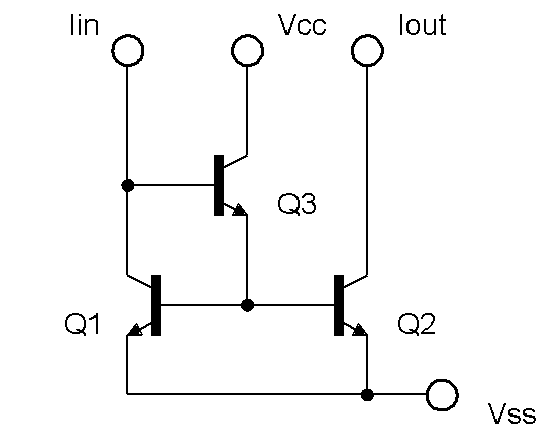
\includegraphics[scale=0.5]{obrazky/ZlepseneWilsonovoZrcadloNPN}
  \end{center}
  \caption{Zlepšené Wilsonovo proudové zrcadlo.}
\end{figure}

Pro sazbu vektorových obrázků přímo v~\LaTeX{}u je možné doporučit balíček \href{https://www.ctan.org/pkg/pgf}{\texttt{TikZ}}.
Příklady sazby je možné najít na \href{http://www.texample.net/tikz/examples/}{\TeX{}ample}.
Pro vyzkoušení je možné použít programy QTikz nebo TikzEdt.




\chapter{Příklad sazby zdrojových kódů}

\section{Balíček \texttt{listings}}

Pro vysázení zdrojových souborů je možné použít balíček \href{https://www.ctan.org/pkg/listings}{\texttt{listings}}.
Balíček zavádí nové prostředí \texttt{lstlisting} pro sazbu zdrojových kódů, jako například:
%
\begin{lstlisting}[language={[LaTeX]TeX}]
\section{Balíček lstlistings}
Pro vysázení zdrojových souborů je možné použít
	balíček \href{https://www.ctan.org/pkg/listings}%
	{\texttt{listings}}.
Balíček zavádí nové prostředí \texttt{lstlisting} pro
	sazbu zdrojových kódů.
\end{lstlisting}
%
Podporuje množství programovacích jazyků.
Kód k~vysázení může být načítán přímo ze zdrojových souborů.
Umožňuje vkládat čísla řádků nebo vypisovat jen vybrané úseky kódu.
Např.:

\noindent
Zkratky jsou sázeny v~prostředí \texttt{seznamzkratek}:
\label{lst:zkratky}
\lstinputlisting[language={[LaTeX]TeX},nolol,numbers=left,firstline=1,lastline=1]{text/zkratky.tex}
%
Šířka textu druhého parametru \verb|KolikMista| udává šířku prvního sloupce se zkratkami.
Proto by měla být zadávána nejdelší zkratka nebo symbol.
Příklad definice zkratky \zk{symfvz} je na výpisu \ref{lst:symfvz}.

\iflanguage{czech}{\shorthandoff{-}}{}
\iflanguage{slovak}{\shorthandoff{-}}{}
\lstinputlisting[language={[LaTeX]TeX},frame=single,caption={Ukázka sazby zkratek},label=lst:symfvz,numbers=left,linerange={bsymfvz-\%\%\%\ esymfvz},includerangemarker=false]{text/zkratky.tex}
\iflanguage{slovak}{\shorthandon{-}}{}
\iflanguage{czech}{\shorthandon{-}}{}

\noindent
Ukončení seznamu je provedeno ukončením prostředí:
\lstinputlisting[language={[LaTeX]TeX},nolol,numbers=left,firstnumber=22,linerange=22]{text/zkratky.tex}

\vspace{\fill}

\noindent
{\bf Poznámka k~výpisům s~použitím volby jazyka \verb|czech| nebo \verb|slovak|:}\newline
Pokud Váš zdrojový kód obsahuje znak spojovníku \verb|-|, pak překlad může skončit chybou.
Ta je způsobená tím, že znak \verb|-| je v~českém nebo slovenském nastavení balíčku \verb|babel| tzv.\ aktivním znakem.
Přepněte znak \verb|-| na neaktivní příkazem \verb|\shorthandoff{-}| těsně před výpisem a hned za ním jej vraťte na aktivní příkazem \verb|\shorthandon{-}|.
Podobně jako to je ukázáno ve zdrojovém kódu šablony.


\clearpage

%\section{Výpis kódu prostředí Matlab}
Na výpisu \ref{lst:priklad.vypis.kodu.Matlab} naleznete příklad kódu pro Matlab, na výpisu \ref{lst:priklad.vypis.kodu.C} zase pro jazyk~C.

\lstnewenvironment{matlab}[1][]{%
\iflanguage{czech}{\shorthandoff{-}}{}%
\iflanguage{slovak}{\shorthandoff{-}}{}%
\lstset{language=Matlab,numbers=left,#1}%
}{%
\iflanguage{slovak}{\shorthandon{-}}{}%
\iflanguage{czech}{\shorthandon{-}}{}%
}

\begin{matlab}[frame=single,float=htbp,caption={Příklad Schur-Cohnova testu stability v~prostředí Matlab.},label=lst:priklad.vypis.kodu.Matlab,numberstyle=\scriptsize, numbersep=7pt]
%% Priklad testovani stability filtru

% koeficienty polynomu ve jmenovateli
a = [ 5, 11.2, 5.44, -0.384, -2.3552, -1.2288];
disp( 'Polynom:'); disp(poly2str( a, 'z'))

disp('Kontrola pomoci korenu polynomu:');
zx = roots( a);
if( all( abs( zx) < 1))
    disp('System je stabilni')
else
    disp('System je nestabilni nebo na mezi stability');
end

disp(' '); disp('Kontrola pomoci Schur-Cohn:');
ma = zeros( length(a)-1,length(a));
ma(1,:) = a/a(1);
for( k = 1:length(a)-2)
    aa = ma(k,1:end-k+1);
    bb = fliplr( aa);
    ma(k+1,1:end-k+1) = (aa-aa(end)*bb)/(1-aa(end)^2);
end

if( all( abs( diag( ma.'))))
    disp('System je stabilni')
else
    disp('System je nestabilni nebo na mezi stability');
end
\end{matlab}

\noindent
\begin{minipage}{\linewidth}


%\section{Výpis kódu jazyka C}

\begin{lstlisting}[frame=single,numbers=right,caption={Příklad implementace první kanonické formy v~jazyce C.},label=lst:priklad.vypis.kodu.C,basicstyle=\ttfamily\small, keywordstyle=\color{black}\bfseries\underbar,]
// první kanonická forma
short fxdf2t( short coef[][5], short sample)
{
	static int v1[SECTIONS] = {0,0},v2[SECTIONS] = {0,0};
	int x, y, accu;
	short k;

	x = sample;
	for( k = 0; k < SECTIONS; k++){
		accu = v1[k] >> 1;
		y = _sadd( accu, _smpy( coef[k][0], x));
		y = _sshl(y, 1) >> 16;

		accu = v2[k] >> 1;
		accu = _sadd( accu, _smpy( coef[k][1], x));
		accu = _sadd( accu, _smpy( coef[k][2], y));
		v1[k] = _sshl( accu, 1);

		accu = _smpy( coef[k][3], x);
		accu = _sadd( accu, _smpy( coef[k][4], y));
		v2[k] = _sshl( accu, 1);

		x = y;
	}
	return( y);
}
\end{lstlisting}
\end{minipage}







\chapter{Obsah přiloženého CD}
Nezapomeňte uvést, co čtenář najde na přiloženém médiu.
Je vhodné okomentovat obsah každého adresáře, specifikovat, který soubor obsahuje důležitá nastavení, který soubor je určen ke spuštění atd.
Také je dobře napsat, v~jaké verzi software byl kód testován (např.\ Matlab 2010b).

Pokud je souborů hodně a jsou organizovány ve více složkách,  je možné pro výpis adresářové struktury použít balíček \href{https://www.ctan.org/pkg/dirtree}{\texttt{dirtree}}.

{\small
%
\dirtree{%.
.1 /\DTcomment{kořenový adresář přiloženého CD}.
.2 loga\DTcomment{loga školy a fakulty}.
.3 FEKT-spec-color.eps.
.3 FEKT-spec-color.pdf.
.3 logolink-op\_vavpi.png.
.3 RE-spec-color.eps.
.3 RE-spec-color.pdf.
.3 SIX\_logo\_zahlavi.png.
.2 obrazky\DTcomment{ostatní obrázky}.
.3 soucastky.eps.
.3 soucastky.png.
.3 spoje.eps.
.3 spoje.png.
.3 ZlepseneWilsonovoZrcadloNPN.eps.
.3 ZlepseneWilsonovoZrcadloNPN.png.
.3 ZlepseneWilsonovoZrcadloPNP.eps.
.3 ZlepseneWilsonovoZrcadloPNP.png.
.2 pdf\DTcomment{pdf stránky generované informačním systémem}.
.3 student-desky.pdf.
.3 student-titulka.pdf.
.3 student-zadani.pdf.
.2 text\DTcomment{zdrojové textové soubory}.
.3 literatura.tex.
.3 prilohy.tex.
.3 reseni.tex.
.3 uvod.tex.
.3 vysledky.tex.
.3 zaver.tex.
.3 zkratky.tex.
.2 navod-sablona\_FEKT.pdf\DTcomment{návod na používání šablony}.
.2 obhajoba.tex\DTcomment{hlavní soubor pro sazbu prezentace k~obhajobě}.
.2 readme.txt\DTcomment{soubor s~popisem obsahu CD}.
.2 sablona.tex\DTcomment{hlavní soubor pro sazbu kvalifikační práce}.
.2 thesis.sty\DTcomment{balíček pro sazbu kvalifikačních prací}.
}
}

%% Konec dokumentu
\end{document}
